\chapter{ライフログ研究の展開と生活状態モデルの数理的基盤}
\label{chap:related-work}

生活状態の理解には、計測可能な行動と本人が経験する主観状態を、異なる種類の情報として扱う必要がある。歩数は身体活動の一側面を表すが、同じ歩数でも活動の目的、作業の内容、疲労の感じ方は異なる。ライフログ研究は、このような生活の記録を複数の情報源から蓄積し、検索、振り返り、状態理解へ利用する研究領域である。本研究は、研究用キーボードを中心とした異種時系列、自己報告、多時間尺度の表現学習、記録の由来を保持する情報モデルを組み合わせる。その基盤を、観測の意味と数理的な操作の両面から整理する。

主構成は、共有三階層LSTMからPlace、Behavior、現在・日次5尺度を得る\texttt{life-discovery-v1}である。本章では、その共通基盤に加え、従来構成のGrowingMap、回答履歴による条件付け、二段階SSL、部分プーリングおよびPMTTを、背景・比較条件として残す。従来構成の数理を提案方式の実装仕様と混同せず、新方式の定式化は第\ref{chap:model}章で行う。

\section{歩数計測と活動量評価}

歩数は、日常の身体活動を時間区間ごとの非負の量へ要約する指標である。Tudor-Lockeらは成人の歩数と身体活動水準の関係を整理しているが、歩数のみからすべての運動強度や活動様式を評価できるわけではない \autocite{tudorlocke2011steps}。歩行、階段移動、自転車運動などでは、同じ時間でも歩数の増え方とエネルギー消費の関係が異なる。生活支援で歩数を利用する際には、測定装置が観測した量、本人の普段の量、推奨する行動を別々に定義する必要がある。

従来構成では、一律の目標歩数への距離だけでなく、同じ参加者が同じ生活状態にいた過去日の歩数との差を用いる。普段から移動が多い状態と机上作業が中心の状態では、比較の基準が異なるためである。この比較は本人の生活内での相対的な不足を表し、身体活動指針への適合や健康状態の診断を直接表すものではない。提案方式の新しいBehavior状態への接続は未検証であり、現行のdiscovery経路ではこの状態別歩数基準による自動提案を停止する。

\subsection{身体活動の連続計測}

参加者\(p\)の累積歩数を\(P_p(t)\)、集約区間を\(I_k=(t_{k-1},t_k]\)とすると、端末が同じ日内で連続して累積値を返す場合、区間歩数は

\[
\Delta P_{p,k}=\max\{0,P_p(t_k)-P_p(t_{k-1})\}
\]

と表せる。日付の切替えや端末変更による累積値のリセットは、通常の増分と分けて処理する。区間長を\(\Delta t_k\)とすると、\(\Delta P_{p,k}/\Delta t_k\)は区間内の平均的な歩数増加率である。ただし、これは連続した歩行中のケイデンスとは異なり、停止や端末を携帯しない時間を含む。日集計は量の比較に適する一方、短い区間の集計は移動が生じた時点を捉える。

計測値\(u_{p,k}\)と観測マスク\(m_{p,k}\in\{0,1\}\)を対にして保持すると、区間に値が存在するかを明示できる。\(m_{p,k}=0\)の区間へ計算上のゼロを入れても、そのゼロを無活動の実測値として扱ってはならない。端末を置いたまま過ごした時間と実際に静止していた時間は、歩数の記録だけでは区別できないからである。観測可能性を確認する補助情報と、活動量を表す値には異なる役割を与える。

歩数を時間へ換算する場合も仮定が必要である。CADENCE-Adults研究は成人の歩行ケイデンスと活動強度の関係を検討している \autocite{tudorlocke2019cadence}。従来構成で用いる100歩/分は運動提案候補を作るための共通換算値であり、全参加者の実測速度を意味しない。METsによる活動間の換算も、身体活動の代表値を用いた概算である \autocite{ainsworth2011compendium}。

\subsection{複数情報源による活動量の文脈化}

歩数の増加が観測された区間に、予定、端末操作、環境イベントを対応付けると、単一の活動量指標に時間的な文脈を与えられる。例えば、予定のある時間帯と端末操作が続く時間帯を区別できれば、同じ低歩数でも異なる生活状況として扱う余地が生まれる。ただし、予定は実行された行動を保証せず、キーボード操作は操作のない時間の活動を直接示さない。センサが示す開閉も、本人の在室や移動を確定する証拠ではない。

異種情報源の統合を\(\boldsymbol{x}_{p,k}=\Phi(\mathcal{E}_{p}^{(1)},\ldots,\mathcal{E}_{p}^{(S)};I_k,t)\)と表す。\(\mathcal{E}_{p}^{(s)}\)は情報源\(s\)のイベント集合、\(\Phi\)は区間集約、\(t\)は推定時点である。イベントの発生時刻だけでなく受信時刻も\(t\)以前である記録から特徴を作ることで、後から届いた情報が過去の推定に混入することを防ぐ。各情報源の集約方法は同一である必要はない。LSTMの歩数特徴には鮮度条件を満たす最新の累積値を使い、従来構成の状態内歩数計算には累積値の増分を使う。操作は回数や間隔、センサは状態、予定は区間との重なりとして表現し、歩数の入力特徴と支援用の集計量を区別する。

この文脈化で重要なのは、複数の値が揃うことよりも、各値の意味と利用可能な時点が揃うことである。すべての情報源を提供した参加者だけを対象とすると、任意同意という観測設計から外れる。したがって、補助情報はマスクとともに入力し、情報源が欠けた条件も独立した評価対象とする。

\section{活動量計測からライフログ研究への発展}

Gurrinらは、個人の生活に関する継続的な記録を、個人の大規模な情報資源として位置付け、取得、管理、検索、利用に関する課題を整理している \autocite{gurrin2014lifelogging}。ライフログは単なる日集計より広く、出来事の順序、時間、場所に関する文脈や、複数の情報の関連を含む。記録を後から振り返る利用と、現在の状態を推定して支援する利用では、必要な時間的制約が異なる。振り返りでは後から追加された情報を使える場合があるが、現在推定の評価では、その時点で受信されていなかった情報を使えない。

本研究の対象は生活全体の完全な記録ではなく、同意された情報源から得られる部分的な記録である。この限定により、観測されていない出来事をモデルが説明したように見せることを避ける。推定モデルには観測の組合せから規則性を学ぶ役割を与え、本人回答には機械的に測定できない主観的な評価を供給する役割を与える。

\subsection{ライフログの観測対象と時間尺度}

観測対象は、身体活動、端末操作、文章特徴、予定、環境状態、自己報告に分けられる。身体活動と操作は連続または短い区間の量として得られ、予定は比較的長い区間を持ち、主観回答は離散的な時点や対象区間を指す。この差を無視してすべてを日平均にすると、短時間の変化が失われる。一方、すべてを最小時間粒度へ展開すると、長い欠測区間と同じ予定の繰返しが系列の大部分を占める。

そこで、細かな観測区間、作業時間枠、日、複数日の履歴を別の単位として扱う。観測窓から時間枠への写像を\(\pi_1(k)\)、時間枠から日への写像を\(\pi_2(u)\)とすれば、情報を要約する演算\(A_1,A_2\)は

\[
\boldsymbol{r}_{p,u}
=A_1\bigl(\{\boldsymbol{x}_{p,k}:\pi_1(k)=u\}\bigr),\qquad
\boldsymbol{d}_{p,d}
=A_2\bigl(\{\boldsymbol{r}_{p,u}:\pi_2(u)=d\}\bigr)
\]

と表せる。平均や和による要約は順序を保持しないため、本研究ではLSTMの最終隠れ状態を用いて順序依存の要約を得る。集約単位は生理的な周期を確定するものではなく、記録の密度と実装上の時間整列に合わせた表現単位である。

\subsection{主観状態の取得と回答負担}

経験サンプリングおよびEcological Momentary Assessment（EMA）は、日常生活の中で繰り返し自己報告を取得する方法である。過去をまとめて回想する評価に比べ、出来事と報告の時間的な近さを保つことを目的とする \autocite{stone1994momentary,shiffman2008ema}。ただし、短時間で回答できることと継続的な負担が小さいことは同義ではない。通知頻度、項目数、中断される作業、回答できる時間帯が、参加者の行動と回答可能性に関わる。

質問\(q\)の提示時刻を\(t_q^{\mathrm{show}}\)、回答時刻を\(t_q^{\mathrm{answer}}\)、対象時刻を\(t_q^{\mathrm{target}}\)とする。回答所要時間\(t_q^{\mathrm{answer}}-t_q^{\mathrm{show}}\)と、対象状態からの遅延\(t_q^{\mathrm{answer}}-t_q^{\mathrm{target}}\)は異なる指標である。前者が長くても、通知を開くまでの待機時間が原因かもしれない。後者が長い場合は、現在値への回答なのか過去状態の回想なのかを区別する必要がある。画面が開かれた時刻を取得できる場合には、提示から開封までと開封から回答までを分けて扱う。

質問頻度と項目数が負担や遵守に与える影響は、EMAの方法研究でも検討されている \autocite{eisele2022burden}。本研究では回答率だけで負担の大小を結論付けず、提示数、回答数、回答遅延、項目別の欠測、継続日数を併記する。未回答は欠測ラベルであり、状態が平均的であったというラベルではない。また、回答しやすい状態が選択的に残る可能性があるため、推定誤差は自己報告が得られた場面に条件付けられた指標として解釈する。

% 追加: FSS発表を入力接点に関する先行検討として位置付ける節。
\subsection{著者の先行検討：生活状態の意味を確認する入力接点と母音省入力インタフェース}

本節は、田中・久保田が第42回ファジィシステムシンポジウム（FSS2026）で発表した「大規模言語モデルを用いた人にやさしい母音ベース省入力日本語インタフェース」 \autocite{tanaka2026fss}を、本修論の研究全体との関係が分かるよう再構成したものである。本修論では、この研究を、観測だけでは確定できない生活状態の意味を本人に確認し、記録するための入力接点に関する先行検討として位置付ける。FSSで評価した対象は文章入力の方式であり、生活状態の確認や生活パターン発見を評価した実験とは区別する。

歩数や端末操作から得られる観測は、生活の一側面を表す。同じ場所で似た操作が続いても、本人にとって同じ作業であるか、異なる作業として区別すべきかは確定しない。生活パターンの候補を本人が確認し、名前を付け、必要に応じて訂正する際には、その判断を受け取る接点が必要となる。前節の自己報告と同様に、この接点では取得できる情報の内容と回答の負担を併せて考える必要がある。

本人確認には選択式の回答も利用できるが、候補への命名や意味の説明、記録の訂正には文字入力を伴う場合がある。そこで問題になるのは、確認に必要な意味を保持しながら、利用者が行う入力操作をどこまで減らせるかである。FSS研究は、高齢者や身体的制約のある利用者、小型端末の利用も想定し、幅広い利用者が少ない負担で意思を伝えられる入力方法を設計目標とした。この目標の下で、キーの選択と方向操作を簡略化する方式を検討した。

日本語入力では、キー位置を選ぶ操作、フリック方向の押し分け、候補を探索する操作などが必要となる。入力記号を少なくすればキーを大きく配置する余地が生まれる一方、区別に必要な情報も失われる。FSS研究が扱った課題は、この情報の損失を候補生成で補いつつ、操作の削減と、利用者が入力内容を変換・確認する負担を分けて調べることであった。

方式は、日本語の5母音と撥音に対応する a、i、u、e、o、n の6記号を入力し、その列から日本語の候補文を生成するものである。例えば「ありがとう」は a i a o u として入力する。6記号という数は文字入力に用いる記号の種類を表し、削除、確定、候補選択まで含めた全操作の種類を表すものではない。試作キーボードでは、これらの記号を中心にキーを配置し、母音列の入力と候補の選択を行える構成とした。

学習用の母音列は、漢字を含む文章を読みへ変換し、各かなを対応する母音へ写像して生成する。撥音は n とし、拗音は一つの母音に集約し、促音や長音記号などは出力しない。この処理では子音や濁音の区別が失われ、「寒い」と「暑い」のように、異なる表現が同じ a u i に対応する。本方式は、この曖昧さを持つ入力から複数の候補を提示し、利用者が意図に照らして選択する入力支援である。

候補生成にはMiniCPM4-0.5Bを用い、LoRAによって母音列から日本語文を生成する課題へ追加学習した。LoRAでは、事前学習済みの重みを固定し、低ランクの更新行列を学習する。母音列に加え、任意の直前文を文脈情報CTXとして与えることで、同じ母音列に対応する表現を文脈に応じて候補化する。推論ではビーム探索を用い、生成結果の重複を除いて上位候補を提示する。基準条件のビーム幅は8、最大新規トークン数は64である。

学習データはCC-100日本語版、OpenSubtitles日本語、JESCから構築した。2〜20字の日本語文を対象に、母音列、同一原文内の直前文、正解文の組を作り、学習750,029件、評価1,497件とした。学習時にはCTXを確率的に除去し、文脈がない条件も扱う。オフライン評価では、数字・英字を含む文を除いた1,378文を用いた。こうした選別条件を持つ評価であり、日常の自由記述全般を同じ条件で扱えたことを意味しない。

% TODO: 図ファイルは FSS 論文から抽出・再構成して追加すること。追加したら次の行のコメントを外す。
\begin{figure}[tbp]
  \centering
  % \includegraphics[width=\linewidth]{figures/fig_fss_overview.png}
  \caption{母音省入力方式の概要。田中・久保田 \autocite{tanaka2026fss}を基に再構成。}
  \label{fig:fss-overview}
\end{figure}

% TODO: 図ファイルは FSS 論文から抽出・再構成して追加すること。追加したら次の行のコメントを外す。
\begin{figure}[tbp]
  \centering
  % \includegraphics[width=\linewidth]{figures/fig_fss_keyboard.png}
  \caption{試作した母音キーボードの画面。田中・久保田 \autocite{tanaka2026fss}を基に再構成。}
  \label{fig:fss-keyboard}
\end{figure}

オフライン評価では、入力記号を減らす効果と、日本語候補の生成性能を別々に測った。入力効率には、誤りなく入力するための最小打鍵数を正解文字数で割る理想KSPCを用いた。各方式の打鍵数は正解文の読みから数え、分母は同一の正解文字数とした。候補生成には、上位k件の候補に正解文全体が含まれる割合Acc@kを用いた。これは文全体の完全一致率であり、意味的に近い候補や一部だけ一致する候補の割合ではない。

表の理想KSPCは、母音IMEが1.12、ローマ字入力が1.95、JISかな入力・フリック入力が1.34、トグル入力が3.06であり、この評価集合では母音方式の必要打鍵数が少なかった。ただし、理想KSPCには誤入力の訂正や候補探索・選択を含めていない。キー数の減少、理想的な打鍵数の減少、実際の回答負担の軽減はそれぞれ異なる評価対象である。

\begin{table}[tbp]
  \centering
  \caption{理想入力効率と候補生成の主要結果。田中・久保田 \autocite{tanaka2026fss}の表3・4を基に再構成。評価対象はいずれも1,378文である。}
  \label{tab:fss-results}
  \begin{tabular}{lll}
    \hline
    評価 & 条件・方式 & 結果 \\
    \hline
    理想KSPC & 母音IME & 1.12 \\
    理想KSPC & ローマ字入力 & 1.95 \\
    理想KSPC & JISかな入力・フリック入力 & 1.34 \\
    理想KSPC & トグル入力 & 3.06 \\
    完全一致率・応答時間 & CTXあり、ビーム幅8、LoRAあり & Acc@1＝7.0\%、Acc@3＝11.8\%、Acc@5＝14.1\%、694 ms \\
    完全一致率 & CTXなし、ビーム幅8、LoRAあり & Acc@5＝12.2\% \\
    完全一致率・応答時間 & CTXあり、ビーム幅16、LoRAあり & Acc@5＝15.2\%、979 ms \\
    完全一致率 & LoRAなし & Acc@1・Acc@3・Acc@5はいずれも0.0\% \\
    \hline
  \end{tabular}
\end{table}

基準条件ではAcc@1が7.0\%、Acc@3が11.8\%、Acc@5が14.1\%であり、候補数を増やすと完全一致率は上がるものの、正解文を候補に含められない例が多く残った。CTXなしのAcc@5は12.2\%で、直前文を利用した条件が上回った。LoRAなしではAcc@1、Acc@3、Acc@5がすべて0\%であり、この実験条件では追加学習が候補生成に必要であった。ただし、これらは指定したモデルと評価集合に関する結果である。

ビーム幅8ではAcc@5が14.1\%、応答時間が694 msであったのに対し、幅16では15.2\%、979 msとなった。探索を広げることによる完全一致率の改善と待ち時間の増加が併存している。応答時間は母音列を入力してから候補が提示されるまでの推論時間であり、利用者が文を考えたり候補を選んだりする時間まで含めた回答所要時間とは異なる。

利用者実験は5名による予備実験であり、9文の課題をひらがな入力、母音入力、標準IME、母音IMEの4方式で比較した。課題は単語、10文字以内の短文、一般文の段階からなり、提示文を一定時間後に隠して、記憶した内容を入力する形式とした。推論なしの比較ではひらがな入力と母音入力を、推論ありの比較では標準IMEと母音IMEを比較することで、母音列への変換と候補提示を分けて検討した。

入力時間は、正答試行のみを集計した参加者平均である。推論ありでは標準IMEが6,675 ms、母音IMEが3,489 msであった。この条件で正しく完了した入力について、母音IMEの時間が短いという結果である。誤答や失敗を含む全試行の完遂性能、任意の文章に対する入力速度、母集団での一般的な優位性を表すものではない。5名という規模を踏まえ、論文は母集団レベルの有意差検定を目的とせず、記述的に分析した。

推論なしでは、ひらがな入力が6,495 ms、母音入力が6,040 msであった。打鍵数は14.1から8.2に減った一方、課題文を隠してから最初の打鍵までの初動時間は1,224 msから1,539 msへ増えた。打鍵を少なくしても、入力前に文を母音列へ変換する処理の時間が残ることを示唆する。初動時間には記憶した文の想起なども関わり得るため、認知負担そのものの直接測定値としては扱わない。

\begin{table}[tbp]
  \centering
  \caption{利用者実験の客観指標。田中・久保田 \autocite{tanaka2026fss}の表5を基に再構成。5名の正答試行のみの参加者平均である。「—」は母音IMEで共通の比較対象から外した項目を表す。}
  \label{tab:fss-user-study}
  \begin{tabular}{llrrr}
    \hline
    比較区分 & 方式 & 総入力時間（ms） & 初動時間（ms） & 打鍵数 \\
    \hline
    推論なし & ひらがな入力 & 6,495 & 1,224 & 14.1 \\
    推論なし & 母音入力 & 6,040 & 1,539 & 8.2 \\
    推論あり & 標準IME & 6,675 & 1,100 & 14.9 \\
    推論あり & 母音IME & 3,489 & — & — \\
    \hline
  \end{tabular}
\end{table}

母音IMEは、母音列を入力してから候補を選んで文章を確定する方式である。打鍵がそのまま確定文字になる方式とは操作の意味が異なるため、最終論文では母音IMEの初動時間と打鍵数を共通の比較対象から外した。表中の空欄相当の記号を、操作が不要であることや値がゼロであることと解釈してはならない。また、正答試行に限定した時間比較と、オフラインの完全一致率は、異なる課題と集計条件で得られた指標である。

主観評価は7段階で、1を「全くそう思わない」、7を「非常にそう思う」とする項目への回答を参加者平均として示した。尺度の中点は4であり、標本の中央値とは区別する。最終論文の表6では、操作の難しさが2.4、母音変換の難しさが4.6、混乱・ストレスが5.4、疲労が4.6、候補の有用感が4.4、利用意向が3.2であった。難しさやストレスの項目は値が大きいほど負担への同意が強く、有用感や利用意向とは評価の向きが異なる。

操作の難しさは中点を下回る一方、母音変換の難しさ、混乱・ストレス、疲労は中点を上回った。候補の有用感は中点をわずかに上回るが、利用意向は下回っており、これらをまとめて使いやすさが高いと結論付けることはできない。客観指標と合わせると、打鍵削減の可能性と、母音変換等に伴う認知的負担が併存した予備的な結果として整理できる。参加者間の差もあり、練習による変化や長期間の利用を判断できる実験ではない。

この入力研究から生活状態理解へ関心が広がった経緯は、2026年7月21日・28日のゼミ資料に記録されている。7月21日には、母音入力モデルの開発を通じて、キーボードを日常行動の取得接点として捉えたことが述べられた。7月28日には、センサだけでは判断できない生活状態の意味を本人に確認する接点として利用する構想が示された。ここから、日常の操作を観測する役割と、観測の意味を本人へ確かめる役割を持つ接点として、キーボードを捉え直した研究経緯を説明できる。

本修論への接続は、この入力接点への問題関心と、評価上の課題を引き継ぐことである。第3章3.2節では通常のキーボード操作を観測し、確定した文章から凍結SentenceTransformerで384次元の埋め込みを生成して32次元へ射影する。母音列から日本語候補を生成するFSSのモデルとは、入力と目的が異なる処理である。母音IMEの現行収集系への導入は本修論の実装内容に含めず、その数値を文章特徴や生活状態モデルの性能として用いない。

FSSの入力方式、第4章4.7節で扱う固定24活動分類や独立ContextLSTM等の従来構成、本修論の主提案であるlife-discovery-v1は、それぞれ対象と評価範囲が異なる。主提案は異種観測から生活パターンの候補を得て、本人の同一性確認・命名・訂正と結び付ける。FSSの予備評価は、この候補発見の精度や意味付けの有効性を裏付けるものではなく、本人の関与を受け取る際の入力設計を考える検討材料として扱う。

操作の少なさと継続的な回答のしやすさは同義ではない。母音入力の短期課題から長期の回答率の増減は判断できないが、操作量だけで取得の成立を評価しないという課題を導ける。本修論では、取得の継続性、回答遅延、欠測、主観的負担を分けて主に評価し、パターン発見・状態推定の性能を補助的に検討する。入力接点の検討を背景として、観測による候補生成と本人による意味の確認を結び付ける生活状態モデルへ、研究課題を展開する。

\section{ライフログによる生活状態の表現}

提案方式で生活状態とは、拠点（Place）、個人固有の行動パターン（Behavior）、気分・疲労・ストレス・集中度・眠気の五つの主観尺度、およびこれらの推移を説明する観測上の文脈の組合せである。PlaceとBehaviorは別々の32次元表現と本人確認IDを持ち、現在・日次の五尺度は順序を持つ値として扱う。固定24活動分類は従来構成の教師付き推定であり、提案方式では既存回答を事後の意味注釈と比較に利用する。観測の類似性から得るマップのノードを一つの活動名、感情または診断名へ直結させず、候補の生成、本人による同一性確認、命名を分けて扱う。

\subsection{多時間尺度の状態表現}

短い操作の変化と数日の生活傾向を一つの系列へ入れると、系列長が増える一方で、短い変化が長期情報の中で埋もれることがある。多時間尺度のモデルは、細かな系列を局所表現へ要約し、その表現の系列から日内の文脈を得て、さらに日をまたぐ文脈を統合する。時間尺度を分けることは、各尺度の変化を独立した原因と仮定することではなく、異なる集約範囲を与える設計である。

本研究ではMicro、Meso、Macroの三階層を用いる。Microは5分ビンを最大12個含む最大1時間の区間、Mesoは日内の区間系列、Macroは当週より前の28日分の日特徴と当週のMesoによる日表現列を対象とする。Microの最終状態をMesoの入力へ渡すが、過去28日の日特徴は下位階層を再実行せず、線形変換してMacroへ直接入力する。この経路により、28日分のすべての操作窓を再帰的に処理する必要を抑える。

階層表現を\(\boldsymbol{h}^{\mu}\)、\(\boldsymbol{h}^{\eta}\)、\(\boldsymbol{h}^{\kappa}\)とすれば、上位表現を下位の出力に反映する融合は、例えば\(\boldsymbol{r}=\tanh(W[\boldsymbol{h}^{\mu};\boldsymbol{h}^{\eta};\boldsymbol{h}^{\kappa}]+\boldsymbol{b})\)と表せる。これは上位のセル状態を下位LSTMへ注入する操作ではない。本実装も表現の連結と全結合層による融合を用い、LSTM内部の状態更新とは分けている。

\subsection{トポロジカルマッピングの原理}

プロトタイプによる状態表現では、高次元入力\(\boldsymbol{x}\)を有限個の代表ベクトル\(\boldsymbol{w}_j\)へ対応付ける。完全観測の場合、勝者は\(b=\arg\min_j\|\boldsymbol{x}-\boldsymbol{w}_j\|_2\)である。代表ベクトルは似た観測を要約し、ノード間の関係は状態間の近さや推移を表す。ただし、近さに基づく接続と時間的な移動に基づく接続は、同じグラフでも意味が異なる。

FritzkeのGrowing Neural Gas（GNG）は、入力に対する勝者と第2勝者、代表の誤差蓄積、接続の老化、誤差の大きい領域へのノード挿入などを組み合わせ、固定ノード数を前提としない構造を学習する \autocite{fritzke1995gng}。これは生活状態を可変数の代表で扱う関連研究として参照できる。

従来構成のGrowingMapは、GNGの更新則を再現するものではない。固定の低次元格子や近傍保存の最適化も持たず、表示の座標が学習済みの生活空間を意味するわけではない。「トポロジカル」という呼称は、観測プロトタイプをノードとし、連続する割当てを有向接続として保持する構造を指す。距離による類似性と時間遷移の頻度を明示し、図の近さをモデルの定義へ逆輸入しないことが必要である。提案方式のDiscoveryMapもGNGの実装ではないが、生観測の距離を使うGrowingMapとは異なり、学習された正規化埋め込みのコサイン類似度を使う。両者の更新則を同一視しない。

\subsection{従来構成のGrowingMapによる状態空間の成長}
\label{sec:legacy-growingmap}

以下は生観測特徴を扱う従来構成のGrowingMapの数理である。新方式のPlace・Behavior埋め込みの更新則や閾値ではない。GrowingMapは、閾値ベース逐次プロトタイプマップと時間遷移グラフを組み合わせた手法である。入力の観測座標を\(O(\boldsymbol{x})\)、ノード\(j\)の観測済み座標を\(O(\boldsymbol{w}_j)\)とし、共通座標を\(C_j=O(\boldsymbol{x})\cap O(\boldsymbol{w}_j)\)とする。場所・アクションのラベル対\(\ell\)も一致することを必要条件とし、距離を

\[
d_m(\boldsymbol{x},\boldsymbol{w}_j)=
\begin{cases}
\sqrt{|C_j|^{-1}\displaystyle\sum_{k\in C_j}(x_k-w_{jk})^2},
& |C_j|\ge3\ \land\ \ell(\boldsymbol{x})=\ell(\boldsymbol{w}_j),\\
+\infty,&\text{それ以外}
\end{cases}
\]

と定義する。座標数で除すことで、共通観測の少ない組合せが単に次元数の少なさから近くなることを抑える。特徴は打鍵回数、訂正、休止、周期時刻を尺度調整した値であり、ラベルの異なる観測を数値上の近さだけで同じ状態へまとめない。

最小距離\(d_{\min}\)が半径\(\rho\)以下なら勝者へ割り当て、観測座標\(k\)ごとの回数\(n_{jk}\)を増やして

\[
n_{jk}\leftarrow n_{jk}+1,\qquad
w_{jk}\leftarrow w_{jk}
+\frac{x_k-w_{jk}}{n_{jk}}
\]

と更新する。新規ノードでは観測された座標のみ \(w_{jk}=x_k, n_{jk}=1\) とし、既存ノードで初めて観測された座標も同様に初期化する。未観測座標は更新しない。これは各座標の逐次平均であり、一定の学習率で隣接ノードまで移動させる更新とは異なる。入力の観測座標が3以上あり、ノードがないか\(d_{\min}>\rho\)であり、ノード数が上限未満のとき、入力を代表とする新規ノードを追加する。既定値は\(\rho=0.35\)、上限は256である。上限到達後の新規性の高い観測は遠い勝者へ強制割当てせず、割当て対象外とする。

連続する割当ての両端が割当て済みで、異なる状態 \(a,b\) に属し、時刻差が \(0\le\Delta t\le12\) 時間のときだけ、\(N_{ab}\leftarrow N_{ab}+1\) と状態変更回数を増やす。自己遷移と12時間を超える間隔は集計しない。記録された状態変更先の構成比を

\[
Q_{ab}=\frac{N_{ab}}{\sum_{c\ne a}N_{ac}},\qquad
b\ne a,\quad\sum_{c\ne a}N_{ac}>0
\]

と定義する。この状態変化率は「記録されたAからの状態変更のうち、Bへ移った割合」である。同一状態への滞在を含む任意の次観測の遷移確率ではない。例えば短い間隔でA,A,A,Bと割り当てられた場合、保存される変更はA→Bの1件であり、\(Q_{AB}=1\)となる。分母が0なら未定義とし、0の構成比や一様分布を補わない。従来構成のコードが保存・公開するのは回数であり、構成比はその回数から導出する。未観測の変更が将来も起こり得ないことを意味しない。新方式も異なる状態への変更回数を保持するが、対象は軸別の埋め込みノードであり、時間間隔の上限は1時間である。12時間という従来の条件を新方式へ適用しない。

更新後に同一ラベルの代表間距離が\(\rho/2\)以下となれば、座標別回数による加重平均で統合する。古い安定IDを保持し、削除したIDは別名として解決し、遷移回数を正規IDへ集約する。自己接続は除く。誤差累積による挿入、第2勝者の更新、辺の年齢による削除は行わないため、GNGの結果を本手法の性質として援用できない。

\begin{figure}[tbp]
  \centering
  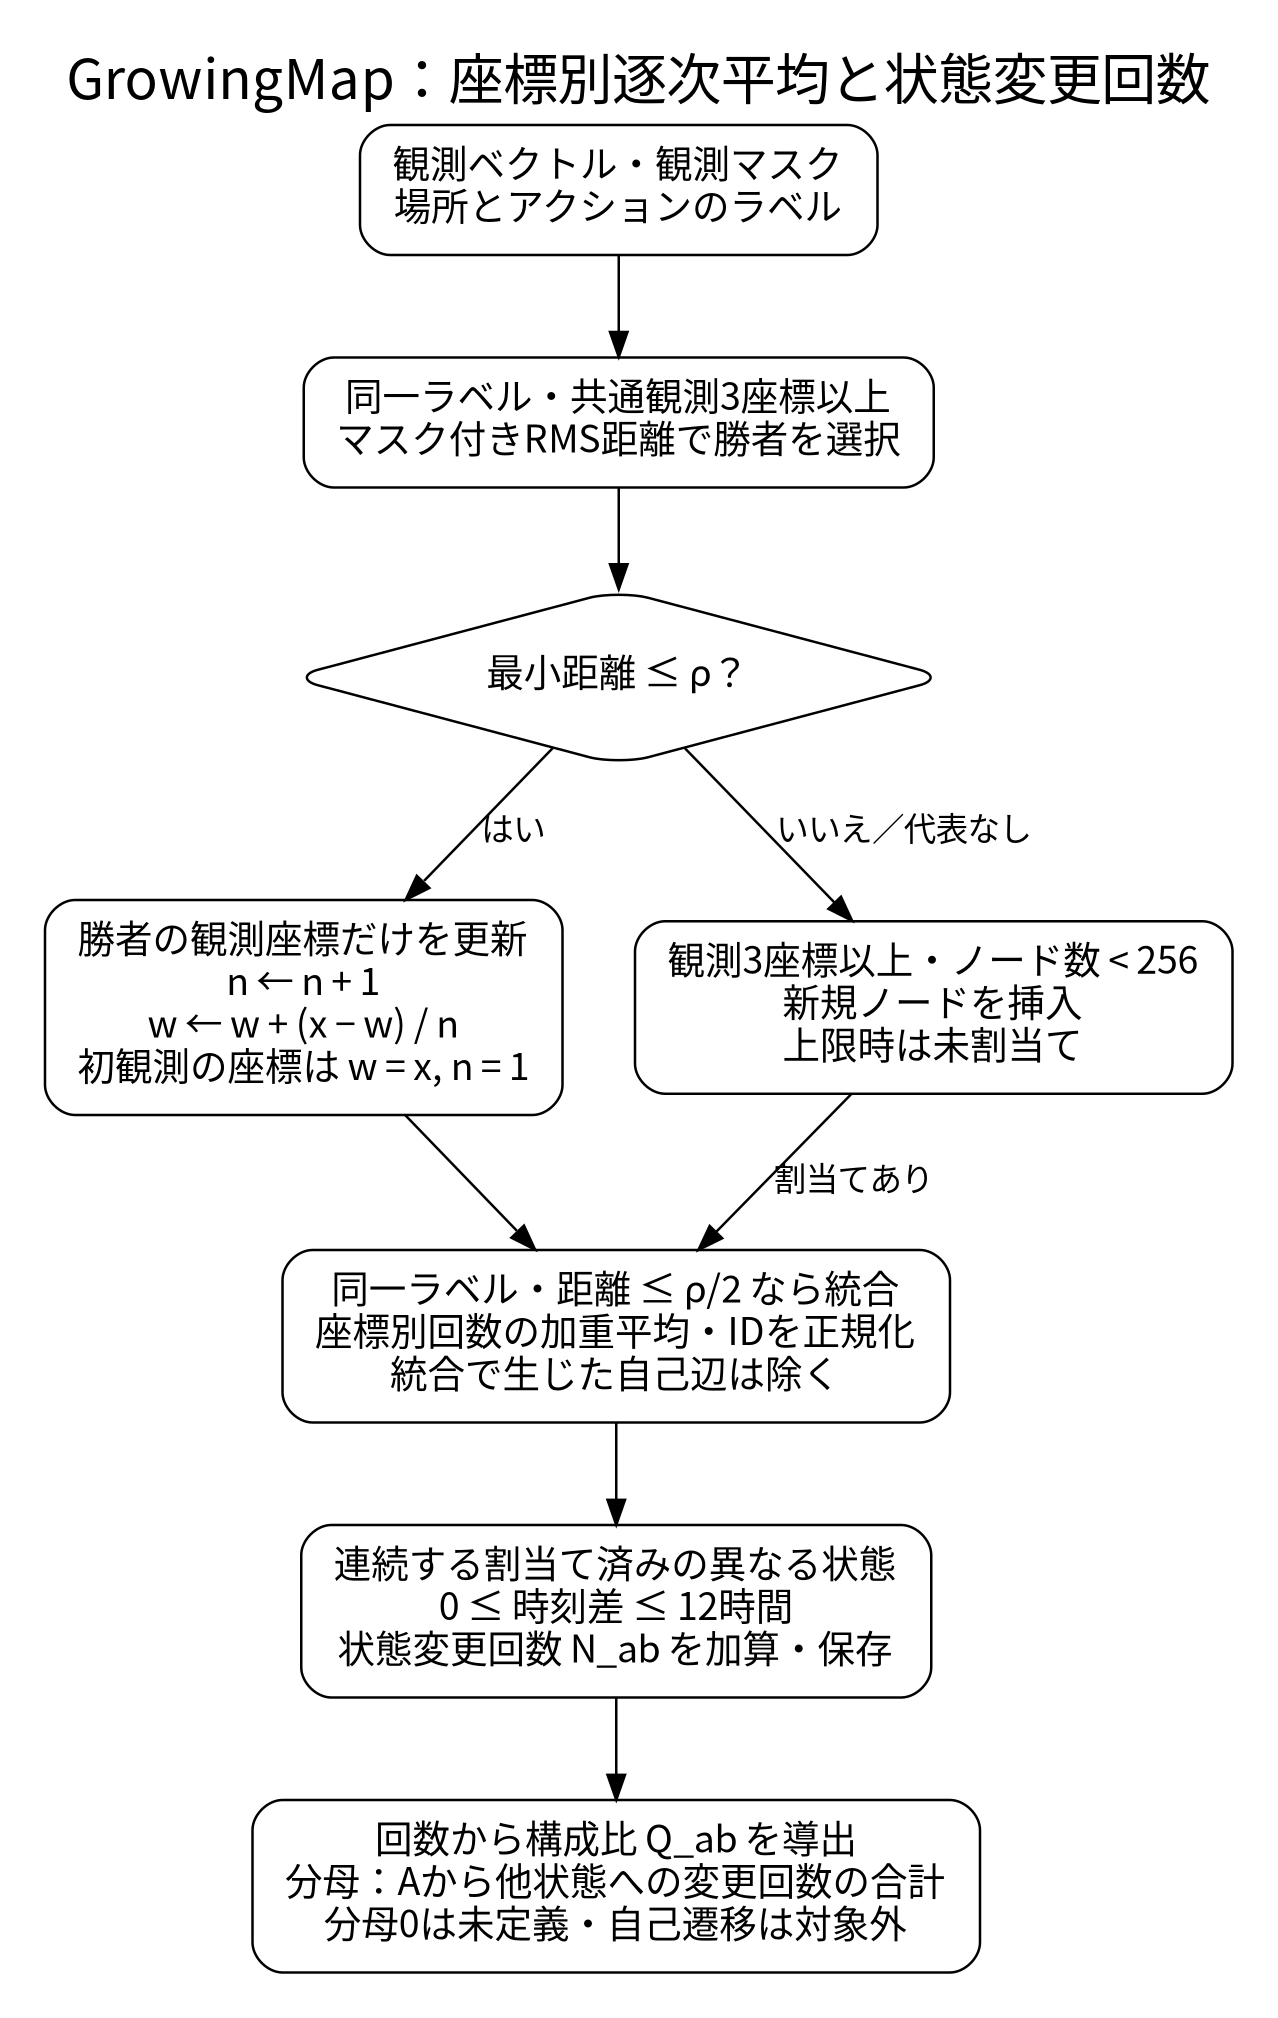
\includegraphics[width=\linewidth,height=180mm,keepaspectratio]{figures/fig_growingmap.png}
  \caption{従来構成のGrowingMapの処理フロー。観測マスクとラベルが一致する代表から勝者を選び、既存ノードの座標別逐次平均更新または閾値による新規ノード生成を行う。図中の矢印は処理順序を示す。状態ノード間の辺には条件を満たす状態変更回数を保存し、構成比は回数から導出する。新方式のDiscoveryMapを示す図ではない。}
  \label{fig:legacy-growingmap}
\end{figure}

\section{時系列推定と個人適応の基盤}

生活状態推定には、入力の時間依存性を表現する学習器と、欠測を除外した教師損失が必要である。本人の履歴による条件付け、逐次重み更新、部分プーリングは、従来構成または拡張比較に属する。表現の記憶、勾配の伝播、推定時に利用できる回答の範囲を別の条件として定義することで、各機構の効果を検証できる。

\subsection{LSTMのゲートとセル状態}

LSTMは、セル状態を通じて過去の情報を保持する再帰型モデルである \autocite{hochreiter1997lstm}。本研究が用いる忘却ゲートを含む形は、初期のLSTMに対する後の発展を含む \autocite{gers2000forget}。入力\(\boldsymbol{x}_t\)、前時点の隠れ状態\(\boldsymbol{h}_{t-1}\)、セル状態\(\boldsymbol{c}_{t-1}\)に対し、各ゲートと候補は

\[
\begin{aligned}
\boldsymbol{i}_t&=\sigma(W_i\boldsymbol{x}_t+U_i\boldsymbol{h}_{t-1}+\boldsymbol{b}_i),\\
\boldsymbol{f}_t&=\sigma(W_f\boldsymbol{x}_t+U_f\boldsymbol{h}_{t-1}+\boldsymbol{b}_f),\\
\boldsymbol{o}_t&=\sigma(W_o\boldsymbol{x}_t+U_o\boldsymbol{h}_{t-1}+\boldsymbol{b}_o),\\
\widetilde{\boldsymbol{c}}_t&=\tanh(W_g\boldsymbol{x}_t+U_g\boldsymbol{h}_{t-1}+\boldsymbol{b}_g),\\
\boldsymbol{c}_t&=\boldsymbol{f}_t\odot\boldsymbol{c}_{t-1}
+\boldsymbol{i}_t\odot\widetilde{\boldsymbol{c}}_t,\\
\boldsymbol{h}_t&=\boldsymbol{o}_t\odot\tanh(\boldsymbol{c}_t)
\end{aligned}
\]

となる。\(\sigma\)はシグモイド関数、\(\odot\)は要素積である。\(W\)は入力から、\(U\)は前の隠れ状態からの重みを表す。PyTorchでは入力側と再帰側に別々のバイアスを持つため、式の\(\boldsymbol{b}\)は両者の和と解釈できる。

入力ゲートは新しい候補を取り込む量、忘却ゲートは過去セルを残す量、出力ゲートはセルを隠れ状態へ読み出す量を制御する。各ゲートは学習されるため、時間が経過すれば必ず一定割合で忘れるという固定規則ではない。セルの加法的な更新経路は過去の情報を保持する助けとなるが、長い依存が常に正確に学習されることを保証しない。系列長、教師信号、最適化、入力の観測密度を併せて評価する必要がある。

\subsection{状態保持とTruncated BPTT}

系列を複数のチャンクへ分けると、順伝播の状態を引き継ぐか、逆伝播をどこまで行うかという二つの選択が生じる。Truncated Backpropagation Through Time（TBPTT）は、時間方向の勾配を有限の範囲へ制限する方法である \autocite{williams1990tbptt}。チャンク\(j\)の最終状態を\(\boldsymbol{s}_{j}^{\mathrm{end}}=(\boldsymbol{h},\boldsymbol{c})\)とし、次の初期状態を

\[
\boldsymbol{s}_{j+1}^{\mathrm{start}}
=\operatorname{sg}(\boldsymbol{s}_{j}^{\mathrm{end}}),\qquad
\frac{\partial\operatorname{sg}(\boldsymbol{s})}{\partial\boldsymbol{s}}=0
\]

とすると、値は保存されるが前チャンクへの勾配は切断される。チャンク損失\(\mathcal{L}_j\)に対する\(\nabla_\theta\mathcal{L}_j\)は、そのチャンク内の計算グラフから計算する。状態をゼロに戻す操作は、値の記憶も失うため、勾配だけを切る操作とは異なる。

従来の状態保持型拡張の比較計画では、Microは同じ作業区間、Mesoは同じ日内という条件下でのみ状態を保持する。参加者の切替え、意味単位の境界、長い欠測では初期化する。Macroは過去28日の明示的な入力窓が長期情報を担うため、チャンク間で状態を持ち越さない。区間・日・週の境界へチャンクを整列させ、境界を越えて異なる意味の状態を連結しない。この状態保持を\texttt{life-discovery-v1}の実装済み設計とは扱わない。

現行の運用コードは、学習例をシャッフルしたミニバッチによるバッチ学習であり、LSTMの初期状態を学習例間で引き継がない。TBPTTおよび逐次状態保持は未実装の比較計画として位置付ける。推論の反復実行、モデルの再学習、LSTM内部状態の持越しは、それぞれ別の処理である。

\subsection{自己報告による個人適応}

個人適応には、過去回答から作る特徴で予測を条件付ける方法と、回答を教師としてモデルの重みを更新する方法がある。従来構成の履歴条件付けは、全履歴、同じ時刻帯、同じ曜日、同じ活動における五尺度の平均と有効性マスクを利用する。特徴\(\boldsymbol{a}_{p,t}\)を変換して表現へ加える操作\(\boldsymbol{r}'_{p,t}=\boldsymbol{r}_{p,t}+g_\theta(\boldsymbol{a}_{p,t})\)は、推論時のパラメータ更新を伴わない。新方式ではこの回答履歴変換を持たず、観測を入力、本人確認と尺度回答を教師として分離する。

重みを更新する個人適応の比較はprequential評価として扱う。時点\(t\)で予測し、その後に受信された回答を将来の更新へ利用する。利用集合を\(\mathcal{A}_p(t)=\{a:t_a^{\mathrm{target}}<t,\ t_a^{\mathrm{received}}<t\}\)とし、同じ回答を繰り返して新規回答として扱わない。遅延回答は対象時点の後でしか利用できず、その回答で更新したモデルを対象時点へ遡って評価すると情報漏洩になる。新方式のライブ推論中にこの重み更新を行う実装はない。

従来構成の比較では、参加者内で学習したモデルを起点とする更新と、条件付けの有無を分ける。全参加者共通の事前学習済みグローバルモデルから個人へ転移する運用機構は存在しない。回答が少ない場合には、重み更新の自由度が高いほど過適合や変動が生じ得るため、凍結条件と更新範囲を制限した条件を同じ予測順序で比較する。

\subsection{自己教師あり学習による表現形成}

自己教師あり学習は、観測自体から学習対象を作り、本人回答がない区間も表現学習へ利用する方法である。BERTはマスクされたトークンの予測を通じて言語表現を学習し \autocite{devlin2019bert}、Masked Autoencodersは画像の一部を隠して再構成する学習を扱う \autocite{he2022mae}。SimCLRは変換した入力間の対比を用いる別の系列の方法である \autocite{chen2020simclr}。これらは自己教師信号の設計例であり、本研究の損失がトークン予測や画像再構成と同一であることを意味しない。

従来構成のSSL実験経路では、観測特徴のランダムマスク再構成と、5〜30分先の特徴予測を組み合わせる。再構成では未観測値を正解にせず、隠した観測座標だけへ誤差を与える。文章埋め込みは意味のまとまりとしてブロック全体を隠し、残った座標から隠れた座標を容易に復元することを抑える。将来予測では入力を時点\(t\)以前へ限定し、教師となる将来特徴を学習区間内から作る。

従来構成の比較計画には、SSL事前学習の後、活動分類と五尺度の教師損失でファインチューニングする二段階学習を含める。事前学習に使うのは対象の参加者データ系列であり、別に存在する全参加者共通モデルを前提にしない。検証・評価期間の未ラベル観測を事前学習へ入れることも、将来情報の利用として排除する。

提案方式では、最新ビンの観測済み特徴を確率0.2で隠す再構成、PlaceとBehaviorからの次1時間の観測予測、本人確認IDの関係損失、現在・日次尺度のHuber損失を同時に最適化する。各埋め込みには縮退を抑える分散項を加える。二段階の事前学習を必須とせず、24クラスの交差エントロピーを含めない。マスクや教師の有効性、係数を含む正確な損失構成は第\ref{chap:model}章\ref{sec:joint-learning}節で示す。

\subsection{階層モデルと部分プーリング}

参加者ごとに完全に別のモデルを学習する方法では、回答数の少ない参加者の推定が不安定になりやすい。一方、全参加者へ同一の平均を当てはめると、尺度の使い方などの個人差を表せない。部分プーリングは、共有構造と個別の効果を組み合わせ、個別効果を共通の中心へ収縮させる考え方である \autocite{gelman2007multilevel}。

五尺度の共有出力を\(f_\theta(\boldsymbol{x}_{p,t})\)、参加者別バイアスを\(\boldsymbol{b}_p\in\mathbb{R}^5\)とすると、

\[
\widehat{\boldsymbol{y}}_{p,t}
=f_\theta(\boldsymbol{x}_{p,t})+\boldsymbol{b}_p,\qquad
\mathcal{J}=\sum_{p,t}\mathcal{L}_{p,t}
+\lambda\sum_p\|\boldsymbol{b}_p\|_2^2
\]

と定式化できる。二乗罰則は、\(\boldsymbol{b}_p\sim\mathcal{N}(\boldsymbol{0},\tau^2I)\)のガウス事前分布に対応するMAP推定の解釈を持つ。従来構成の部分プーリング実験経路では、共有出力と個人バイアスに対する二乗誤差と収縮罰則を用いる。従来基本モデルと提案方式の尺度出力が用いるHuber損失とは区別し、完全な階層ベイズ推論や不確実性の事後分布の計算は行わない。参加者間の部分プーリングは\texttt{life-discovery-v1}には実装されていない。

回答数が少ない個人のバイアスをゼロへ強く制約し、十分な回答がある場合に共有出力からの差を学習する。受信済み回答だけでバイアスを更新する条件、全層を更新する条件、凍結する条件を比較すれば、低い自由度の個人差モデルが逐次評価で安定するかを検討できる。共有エンコーダを実験内で共同学習する設計と、事前に完成したグローバルモデルの存在は区別する。

\section{本人の解釈を保持する情報モデル}

自己報告は、観測の正解を一度だけ付けて完了する操作とは限らない。本人が時間を置いて状態を捉え直したり、推定の誤りを訂正したりするため、記録の対象時点と追加された時点を分けて保持する必要がある。観測、機械推定、提示の根拠、本人の回答を混在させると、どの情報に依存した推定であるかを再現できなくなる。以下では、従来構成のナラティブ記録とPMTTを背景として整理する。情報の役割を分ける考え方は提案方式でも保持するが、PMTTを新しいパターン発見器の一部とはしない。

\subsection{お天気分とナラティブポートフォリオ}

お天気分は、本システムでは本人が主観的な気分を短い選択で表す入力として扱う。入力契約上の値はhappy、normal、sad、angryである。この分類は五尺度の数値回答と異なるため、「happyなら気分5」などの換算をせず、独立した本人の表現として保存する。表現が簡潔であることは、気分のすべての側面が区別されることを意味しない。

ナラティブポートフォリオは、本論文では本人の状態記述、回答、修正を時間順に蓄積し、振り返り可能にする考え方として扱う。特定の外部尺度や標準化された診断法との同等性は前提としない。自由な状態の表現、従来分類の活動カテゴリ、五尺度、提案方式の拠点・行動確認には、異なる情報の粒度がある。提案方式では本人確認と尺度回答を教師に用い、活動回答は事後注釈へ位置付ける。本人の自由な表現をいずれかの教師へ強制的に還元せず保持する。

この設計により、数値は似ていても本人が異なる意味を与えた記録を、同一の経験としてまとめずに済む。また、入力の訂正が増えた理由として誤入力、推敲、変換などを回答できる仕組みは、操作の変化を直ちに疲労と解釈することを避ける助けとなる。本人の解釈を観測値の代わりに用いるのではなく、観測の意味を確認する別の記録として対応付けることが重要である。

\subsection{従来構成のPMTTによる情報の分離}

従来構成のPMTTを記録の由来をたどるグラフ\(G=(V,E_G)\)とする。\(V\)は記録のノード集合、\(E_G\)は関係を表す有向辺集合である。情報の役割を\(\mathcal{O}\)（観測）、\(\mathcal{I}\)（推定）、\(\mathcal{E}\)（根拠）、\(\mathcal{R}\)（本人の回答・修正）で表し、第\ref{chap:model}章の役割表記へ統一する。概念上の対応は

\[
\mathcal{O}\xrightarrow{\mathrm{used\ by}}\mathcal{I},\qquad
\mathcal{E}\xrightarrow{\mathrm{supports}}\mathcal{I}\ \text{または提案},\qquad
\mathcal{R}\xrightarrow{\mathrm{targets}}\mathcal{I}\ \text{または対象区間}
\]

である。役割の分離は、保存上のすべての記録が四種類の専用ノード型を持つことを要求しない。従来APIでは観測、推定、narrative、correctionなどをObservation型で包み、source属性で区別する。これらを毎正時のStateEpisode、Day、月曜起点の固定週Patternへ関連付ける。運動提案はExerciseProposalとして根拠と対応付けられる。この保存の背景は、提案方式で新しい状態に基づく運動提案が実装・検証済みであることを意味しない。

修正記録\(r\in\mathcal R\)は、対象区間、追加時刻、参照ID、修正内容を持つ。元の観測\(o\in\mathcal O\)や推定\(i\in\mathcal I\)を削除して新しい値へ置き換えるのではなく、修正を追加して当時の推定を残す。学習データを作る際に利用可能な修正を選ぶ処理と、履歴の表示は分ける。このため、現在の本人回答と、過去の時点で利用できた本人回答の双方を再構成できる。

PMTTは時間枠に沿う由来の構造であり、未知の行動パターンを自動発見する学習器ではない。GrowingMapの状態ノードとPMTTの時間枠ノードを同一視せず、状態割当てを持つ観測記録を介して対応させる。由来グラフを保持しても、モデルの判断全体が因果的に説明されたことにはならず、どの入力と基準を用いたかという検証可能性を支える。

\section{既存研究の課題と本研究の位置付け}

先行研究から、本研究に関わる課題は三つに整理できる。第一に、異種ライフログの値を時間軸上で統合するだけでは、その値が当時利用できたかを保証できない。イベント時刻と受信時刻の双方を用いた因果カットオフ、任意同意と欠測の区別、ラベル対象区間の定義が必要である。第二に、操作、日内文脈、複数日の履歴を一つの表現へ単純に平均すると、順序と時間尺度の差が失われる。第三に、本人の回答を取得しても、それが推定の上書きとして保存されると、過去の予測と修正の関係を評価できない。

本研究は、研究用キーボードから得る操作特徴とローカル文章特徴を中心に、任意同意の生活情報を加える。文章表現にはSentence-BERTに基づく文埋め込みを利用し \autocite{reimers2019sentencebert}、小型言語モデルの基盤としてMiniLMを参照する \autocite{wang2020minilm}。主条件は研究サーバ上のローカルSentenceTransformerの\path{paraphrase-multilingual-MiniLM-L12-v2}であり、384次元の埋め込みを固定ランダム射影で32次元へ変換する。従来構成と新方式に共通する入力基盤であり、比較時は同一のモデルrevision・内容ハッシュ・射影を固定する。未指定時の文字n-gram経路は別条件である。原文を外部AIサービスへ送らない設計とするが、埋め込み化は個人情報の完全な匿名化を保証する操作ではない。

提案方式は、共有三階層LSTM、Place・Behaviorの独立射影、訓練側で構築するDiscoveryMap、現在・日次5尺度の回帰を主構成とする。自己教師ありの再構成・次1時間予測と本人確認・尺度教師を同時に用い、推論時には重みとマップを凍結する。\texttt{task}はBehaviorの保存・通信上の互換名であり、独立した第三の推定器ではない。

従来の固定24活動分類、独立ContextLSTM、生観測GrowingMap、PMTT、回答履歴条件付け、二段階SSLおよび部分プーリングは、背景・比較条件として保持する。本人平均・前回値などの基準予測との比較も、同じ時点と有効教師にそろえて行う。新方式は\texttt{research\_architecture=discovery}で明示選択し、サーバーの既定は\texttt{legacy}である。主構成の更新と既存運用の切替を区別する。

これらの統合が生活状態推定に有効であるかは、実験前には確定できない。少人数・短期間の予備研究では、取得の継続性と回答負担を主に検討し、推定性能は時間順分割と同一対象での比較により探索的に評価する。理論上の表現力、コードとして実装された処理、評価予定の処理を区別することが、本研究の検証可能な位置付けとなる。
